\chapter{Resultados}
\label{chap:result}
Importante sempre ter um parágrafo introdutório para explicar os resultados encontrados.

%--------- NEW SECTION ----------------------
\section{Robôs Subaquáticos}
\label{underwater_robots}


\subsection{Considerações na Modelagem}
Esta seção aborda os princiapis elementos e considerações para modelagens de ROVs.

Assim como quase todos robôs móveis podem estar posicionado em relação a uma referência, a posição de um robô subaquatico pode ser representando, de acordo com \cite{Antonelli}, diante a sua posição e orientação.
Diante a um Frame fixo de referência, é possivel obter a posição, usando técnicas de sensoriamentom, de um veículo submerso que comunalmente representando como vetor.
%vetor = (x,y,z)

Para representar a rotação dos veiculos diante ao mesmo frame pode usar o vetor
%n =(r,p,y)
que é a representação de roll, pitch  e yaw.

A seguinte tabela apresenta os movimentos dos veículos Subaquáticos em relação ao destes. Esta tabela esta de acordo que demostrado em \cite[Antonelli]. Estes movimentos, surge, sway e heave, também são usados navegações marinhas. 





%lembre de usar o livro de fossen
\subsection{Sensores}

A presença de sensores em um sistema pode permiti a obtenção de dados de vários. A medida dos sensores podem ser direcionados para a propria dinânica de um sistema, neste caso um ROV, e o ambinete no qual este realizar suas ações.
Assim como classifica \cite{Towards}, os sensores de um ROV pode distinguindo em dois grupos: \textit{playload sensors}  e \textit{navigations sensor}. Os \textit{payload sensors} são unidades de medidas destinados a coletar dados do ambiente, alguns exemplos destes sensores saão: sensores CTD, destinados a mensurar a condutividades, temperatura e profundidade, sensores ADCP-Acoustic Doppler Curent pPofiler- são usados para mensurar a velocidade das correntes e câmeras para obter dados visuais.

Os navigations sensors são implementados com o foco na navegação do veículo, logos dados sobre a posição, orientantçã e veocidade são os principais alvos a serem mensurados. Os navigations sensors mais comum são: sensores de pressão, (DVL) mede o deslocamento Doppler no sinal de entrada refletido no fundo do mar para obter os dados da velocidade linear e sensores de inercia. 
Câmeras também podem ser usadas para obter dados da posiação de veículos, assim como foi demostrado por \cite{visual_serving}, no qual foi ultizado duas câmeras par realizar um acomphamento da posição de ROV. Os dados dos sensores podem ser usados para o monitoramento e para as ações de controle.

% Colocar a tabela com as imagens dos principais sensores



\subsection{Controle}
\subsection{Arquitetura de Operação}
Há diversas formas que as arquiteturas de operação diante do nível de autonomia dos ROVs podem ser implementados. Uma comum é quando um humano é responsável 100\% das atuações do veículos, em outras palavras, é aplicado um controle 100\% manual. O operador, neste caso costuma ser um bastante habilidoso, comunalmente usa uma video câmera para estimar a posiação do veículo no ambiente.

% achar uma referência para o controle manual.

Uma arquiteura, segundo \cite{wireless_joy}, é \textit{Human in the Loop} - HITL- que é realizado considerando a arquitetura \textit{Human Centered Automantion} - HCA. Nesta arquitetura o operador humano realizar algumas tarefas do sistema de controle, ao exemplo de selecionar de qual mode de ação de movimento o veiculo deve realizar. Alguns exemplos dos modo de ação o controle de profundidade, heading e seguir tubulações.

Outros tipos de operações são apontadas por \cite{Towards}: \textit{Automatic Operation}, \textit{Management by consent}, \textit{Semi-autonomous or management by exception} e \textit{Highly autonomous}. O primeiro, \textit{Automatic Operation}, possui caracteristicas semelhante ao \textit{human in the loop} e o segundo, \textit{Management by consent} é basicamente uma teleoperação. O \textit{Semi-autonomous or management by exception} é montado para o sistema executar automaticamente as funções relacionadas à missão quando os tempos de resposta são muito curtos para intervenção humana.  Quando não necessidade de um operador realizar nenhuma intervenção sobre o veiculo, o tipo de operação é considerada \textit{Highly autonomous}. Esta última classificação esta mais proxima das condicções necessarios para um veiculo submarino ser considerado um AUV.





\subsection{Modelos de ROVs}

Existem vários modelos de robôs submarinos. O formato deste veículos podem ser em função de diversas considerações. Local de atuação, profundidade onde as atividades serão executadas, suporte para a presença de braços manipuladores.
\subsubsection{BlueROV2}


O BlueROV2, representado na Figura \ref{fig:blue}, é desenvolvido pela Blue robotics, uma comphania americana especilizada em robô submarinos. Assim como informa \cite{Bluerobotics}, este veículo é destinado para realizar inpeções e pesquisas. O alcance de profundidade é de 100 m. 6 thursters são responsáveis pela atuação, 4 lâmpadas, também há versões com 6, e uma camêra HD coletar os dados visuais. 
Além destas configurações, outros intems pode ser adicionados ao exemplo de gripper, para realizar aconrragem, e sonares, para medição de profundidade e escananeamento. Um ponto imporante do Blue Rov é o fato de ROV ser opensource,  que permiti de várias modificações e dominio dos eventuais usuário.

\begin{figure}
  \centering 
  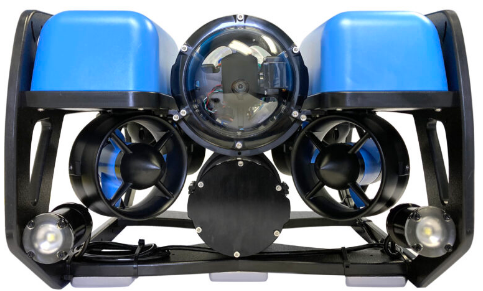
\includegraphics[width=150.5]{blue_rov.png}
  \caption{BlueROV2}
  \label{fig:blue}
\end{figure}

\subsubsection{Freedom ROV}


O Freedom ROV, apresentado na Figura \ref{fig:freedom_rov}, é desenvolvido pela comphania OCEANEERING, dentêm uma como a principal caracteristicas ter modos de operações híbridas. Segundo \cite{Bogue1}, Freedom pode operar sem intermédio de ações humanas, com ou sem a presença de cabos de comunicação. Este veiculo também capacidade de realizar \textit{subsea residence}, que é capacidade dos robôs ficarem alocadod no mar por um perido longo, neste caso seis meses. Durante o periodo de residência submarina, o Freedom ROV realizar o recarregamento de energia em estações de docagem submersas.


\begin{figure}
  \centering 
  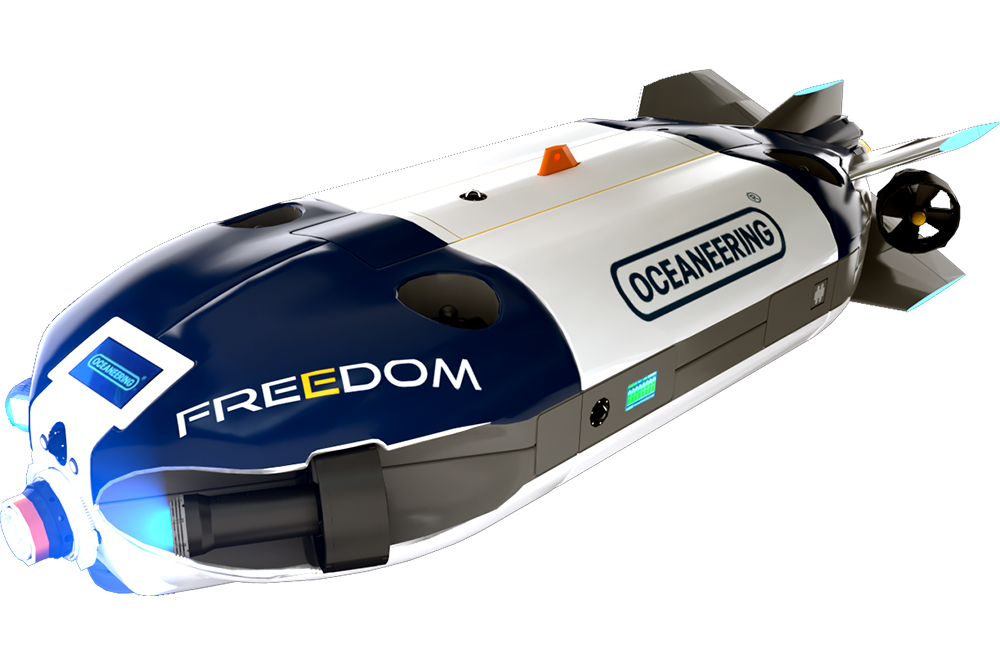
\includegraphics[width=150.5]{freedom_rov.png}
  \caption{Freedom ROV}
  \label{fig:freedom_rov}
\end{figure}

\subsubsection{SEASCAN MK2}


A ECA GROUP, uma companhia franceza especializada em desenvolver veículos marinhos e submarinos, desenvolveu um o ROV SEASCAN MK2, representado na Figura \ref{fig:seascan}. Este robô é tem uma forma de torpedo. De acordo com \cite{ECA_GROUP}, O SEASCAN é um veículo leve e pode ser usado para inspeções, identificação de minas e para missões com fins ambientais. Cabos umbilicais não são usados para nem para cominicação e nem para alimentação.  Uma bateria recarragável é a fonte de alimentação deste robô.

Também é apontado por \cite{ECA_GROUP} que o SEASCAN MK2 também pode realizar algumas duas tarefas autônomas. Uma é dedicada para realizar posicionamento diante a profundidade do veículo, a outra é focada em automatizar o caminho do veículo a alcançar uma area específica.



\begin{figure}
  \centering 
  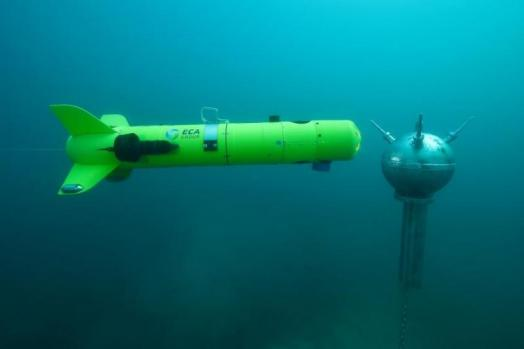
\includegraphics[width=150.5]{seascan.jpg}
  \caption{SEASCAN MK2}
  \label{fig:seascan}
\end{figure}


\subsubsection{Aquant ROV}

O Aquant ROV um é veículo, de acordo \cite{Bogue1}, que além de possuir operação hibrida, autonomo e teleoperado., também não possui um formato único. O Aquant ROV possui dois formatos de operação, um para o modo autonomo, e outro para realizar teleoperação.
A Figura n representa o Aquant na forma autonoma e  a Figura é o foramto que o Aquant adiquiri ao passar para a atuação teleoperado.

O modo de atuação autonoma é realizada até o robô antingir o momento de realizar as atividades destinadas ao trabalhos com manipuladores. Para atuar de forma com os manipuladores, o Aquant mudar de formato e sua atuação passar a ser completamente por fins de teleoperação, em outras palavras há uma necessidade de presenaça  humana na operação. 



\section{Revisão bibliográfica}
\subsection{Rede de Citação}
\subsection{Principais autores}
\section{Mapa COnceitual}
\lipsum[1]

%--------- NEW SECTION ----------------------
\section{Testes integrados}
\label{sec:testi}
\lipsum[1]







